\chapter{Feedback del CSI a tasso variabile}

\thispagestyle{empty}

Detti \(b_\mathrm{F}\) il numero di bit trasmessi in feedforward, ovvero dalla
BS allo UT, e \(b_\mathrm{B}\) il numero di bit trasmessi come feedback, dallo
UT alla BS, definiamo come
\[
    B = b_\mathrm{F} + b_\mathrm{B}
\]
il numero totale di bit scambiati tra BS e UT.

Nella procedura a tasso variabile, illustrata in seguito, imponiamo
\(b_\mathrm{F} = 0\), ovvero nessun bit viene inviato dalla BS allo UT in
feedforward. In particolare, permettiamo al numero di bit di feedback
\(b_\mathrm{B}\) di variare, pertanto la segnalazione di feedback ha un tasso
variabile.

Anzitutto, modelliamo lo scenario considerato come una codifica di sorgente di
due sorgenti correlate (i canali di UL e DL, in questo caso).  Quindi,
dimostreremo che la presenza di una segnalazione di feedforward da parte della
BS non contribuisce a ridurre il tasso medio della segnalazione di feedback,
risultando quindi superflua al fine di ridurre l'overhead complessivo. Infine,
proponiamo una procedura con approccio feedback-only a tasso variabile, basata
sull'entropia condizionale del canale di DL condizionata al canale di DL.

\lipsum[4]  % TODO: add something about the noisy case.

\section{Codifica di sorgenti correlate}

Dal teorema di Shannon sulla codifica di sorgente
\cite{10.1002/j.1538-7305.1948.tb01338.x} è noto che per codificare una
sorgente \(X\), un tasso \(R > \entropy{X}\) è sufficiente. Consideriamo ora
due sorgenti correlate \((X,Y) \sim p(x, y)\). In questo caso, un tasso pari a
\(\entropy{X,Y}\) è sufficiente per codificarle congiuntamente. Supponiamo che
al ricevitore si desideri ricostruire \(X\) e \(Y\) separatamente. Si vede
facilmente che un tasso \(R = R_X + R_Y > \entropy{X} + \entropy{Y}\) è
sufficiente. Tuttavia, Slepian e Wolf \cite{1055037} hanno dimostrato che un
tasso totale pari a \(R = \entropy{X,Y}\) è sufficiente anche per codificare
separatamente le due sorgenti correlate.

Riportiamo nel seguito il teorema di Slepian-Wolf
\cite{10.1002/047174882X.ch15}. In Figura~\ref{fig:sw-configuration} è
illustrata la situazione considerata.

\begin{figure}[ht]
    \centering
    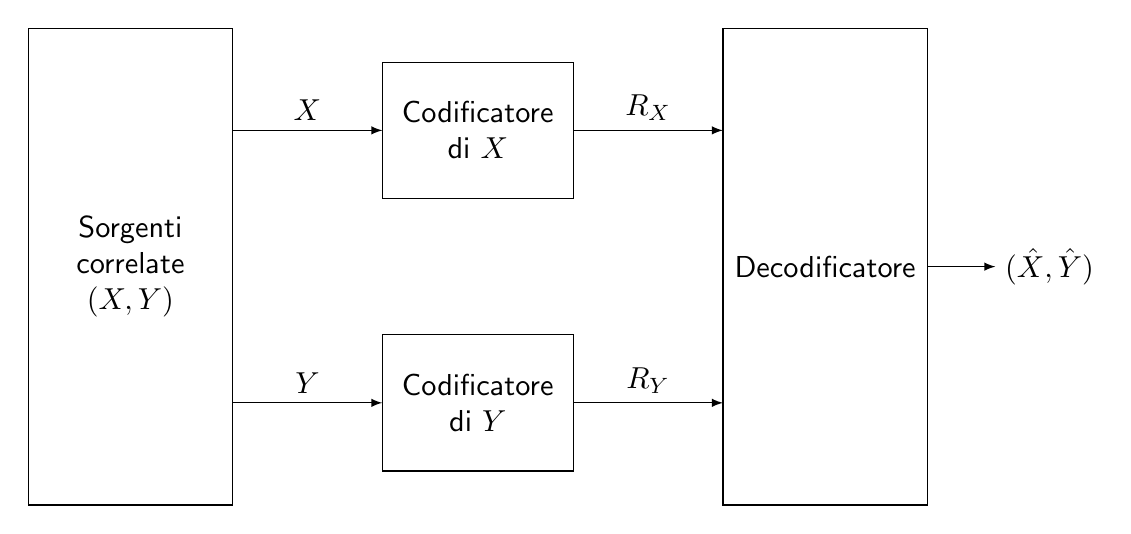
\begin{tikzpicture}[scale=0.865,>=latex]
    \tikzstyle{every node}=[font=\fontsize{11}{13}\sffamily]

    \draw (0,0) rectangle (3,7)
    node[midway,align=center]{Sorgenti \\ correlate \\ \((X,Y)\)};

    \draw[->] (3,5.5) -- (5.2,5.5)
    node[above,midway]{\(X\)};

    \draw[->] (3,1.5) -- (5.2,1.5)
    node[above,midway]{\(Y\)};

    \draw (5.2,4.5) rectangle (8,6.5)
    node[midway,align=center]{Codificatore \\ di \(X\)};

    \draw (5.2,0.5) rectangle (8,2.5)
    node[midway,align=center]{Codificatore \\ di \(Y\)};

    \draw[->] (8,5.5) -- (10.2,5.5)
    node[above,midway]{\(R_X\)};

    \draw[->] (8,1.5) -- (10.2,1.5)
    node[above,midway]{\(R_Y\)};

    \draw (10.2,0) rectangle (13.2,7)
    node[midway]{Decodificatore};

    \draw[->] (13.2,3.5) -- (14.2,3.5)
    node[right]{\((\hat{X},\hat{Y})\)};
\end{tikzpicture}

    \caption{Configurazione per la codifica di sorgente Slepian-Wolf.}
    \label{fig:sw-configuration}
\end{figure}

\begin{thm}[Slepian-Wolf \textnormal{\cite{10.1002/047174882X.ch15}}]
    \label{thm:sw}

    Sia \((X_1,Y_1),(X_2,Y_2),\dots\) una sequenza di variabili aleatorie
    congiunte, indipendenti e identicamente distribuite tali che la generica
    coppia \((X,Y) \sim p(x, y)\).\\
    Per il problema della codifica di sorgenti distribuite per la sorgente
    \((X,Y)\), la regione di tasso raggiungibile è data da
    \begin{alignat}{1}
        R_X &\ge \entropy{X \vert Y}, \label{eq:SW1} \\
        R_Y &\ge \entropy{Y \vert X}, \label{eq:SW2} \\
        R_X + R_Y &\ge \entropy{X,Y}. \label{eq:SWsum}
    \end{alignat}
\end{thm}

La Figura~\ref{fig:sw-rate-region} mostra la regione descritta dal
Teorema~\ref{thm:sw}.

\begin{figure}[ht]
    \centering
    \begin{tikzpicture}[>=latex]
    %\tikzstyle{every node}=[font=\fontsize{11}{13}\sffamily]

    \draw[->] (0,0) -- (8,0)
    node[right]{\(R_X\)};

    \draw[->] (0,0) -- (0,6)
    node[above]{\(R_Y\)};

    \draw (1.8,3pt) -- (1.8,-3pt)
    node[anchor=north]{\(\entropy{X \vert Y}\)};

    \draw (3.6,3pt) -- (3.6,-3pt)
    node[anchor=north]{\(\entropy{X}\)};

    \draw (7.2,3pt) -- (7.2,-3pt)
    node[anchor=north]{\(\entropy{X,Y}\)};

    \draw (3pt,2) -- (-3pt,2)
    node[anchor=east]{\(\entropy{Y \vert X}\)};

    \draw (3pt,3) -- (-3pt,3)
    node[anchor=east]{\(\entropy{Y}\)};

    \draw (3pt,4) -- (-3pt,4)
    node[anchor=east]{\(\entropy{X,Y}\)};

    \draw[help lines] (7.2,0) -- (0,4);
    \draw[help lines] (1.8,0) -- (1.8,5.5);
    \draw[help lines] (3.6,0) -- (3.6,2);
    \draw[help lines] (0,2) -- (7,2);
    \draw[help lines] (0,3) -- (1.8,3);

    \draw (3.6,2) -- (7,2);
    \draw (3.6,2) -- (1.8,3);
    \draw (1.8,5.5) -- (1.8,3);

    \foreach \x in {2.64,2.74,...,6}
    \draw[xslant=0.5] (\x cm,2) -- (\x cm,2.22);

    \foreach \x in {0.2,0.3,...,2.2}
    \draw[rotate=-29.055] (\x cm,3.5) -- (\x cm,3.75);

    \foreach \y in {-0.2,-0.04,...,2.22}
    \draw[yslant=1.8] (1.8,\y cm) -- (1.925,\y cm);

    \draw (4,3.5) node{\(\mathcal{R}\)};
\end{tikzpicture}

    \caption{Regione \(\mathcal{R}\) di tasso raggiungibile con la codifica di
    sorgente Slepian-Wolf.}
    \label{fig:sw-rate-region}
\end{figure}


\section{Approccio feedback-only}

\lipsum[4]


\section{Procedura di codifica}
\label{sec:procedure}

Il Teorema~\ref{thm:feedback-only} mostra che, quando una codifica a tasso
variabile viene utilizzata, è possibile operare un approccio feedback-only.
Proponiamo ora una procedura di codifica basata su quanto descritto da Al Jabri
e Al-Issa.\cite{10.1007/BFb0024445}

Modelliamo il canale di UL come una sorgente discreta di informazione, con
alfabeto \(\set{V}\), che è, di fatto, il codebook utilizzato alla BS per la
rappresentazione locale del canale di UL, con \(\abs{\set{V}} = \gamma =
2^{b_\mathrm{U}}\) parole di codice. Allo stesso modo, modelliamo il canale di
DL come una sorgente discreta di informazione, con alfabeto \(\set{D} =
\set{D}_1\), cioè l'unico codebook di DL possibile (dato che per \(b_\mathrm{F}
= 0\), \(\alpha = 2^{b_\mathrm{F}} = 1\)), avente \(\abs{\set{D}} = \beta =
2^{b_\mathrm{B}}\) parole di codice.

La distribuzione congiunta delle coppie \((\bm{v}_i,\bm{d}_j) \in
\set{V} \times \set{D}\) è descritta dalla matrice di densità di probabilità
discreta congiunta \(\bm{P}\), il cui \((i,j)\)-esimo elemento è
\begin{equation}
    p_{i,j} = p(\bm{v}_i, \bm{d}_j) = \prob{
        q(\bm{h}^\mathrm{(U)}) = \bm{v}_i \:,\;
        q(\bm{h}^\mathrm{(D)}) = \bm{d}_j
    } .
\end{equation}

La sparsità della matrice \(\bm{P}\) aumenta con il crescere di \(B\), di
\(b_\mathrm{U}\), o della correlazione tra UL e DL.

Come descritto da Al Jabri e Al-Issa \cite{10.1007/BFb0024445}, è possibile
minimizzare il tasso di codifica determinando una partizione di \(\set{D}\) che
abbia entropia minima, come illustrato nella procedura seguente.

\begin{enumerate}

    \item Applicare la stessa dimensione di blocco ai due alfabeti, ovvero
        porre \(b_\mathrm{B} = b_\mathrm{U}\).
        \label{itm:alphabets-sizes}

    \item Per ogni \(j,\,j = 1,\dots,\beta\), costruire un sottoinsieme
        \(\set{V}_i\) di \(\set{V}\) tale che
        \begin{equation}
            \set{V}_i = \mleft\{
                \bm{v} \mid \bm{v} \in \set{V} \land
                \bm{d}_j \in \set{D} \land
                p(\bm{v}\given\bm{d}_j)>0
                \mright\}. \label{eq:subsets-of-v-cond}
        \end{equation}
        Si noti che, poiché \(p(\bm{v}\mid\bm{d}_j) =
        \frac{p(\bm{v},\bm{d}_j)}{p(\bm{d}_j)}\), la
        \eqref{eq:subsets-of-v-cond} è equivalente a
        \begin{equation}
            \set{V}_i = \mleft\{
                \bm{v} \mid \bm{v} \in \set{V} \land
                \bm{d}_j \in \set{D} \land
                p(\bm{v},\bm{d}_j)>0
                \mright\}, \label{eq:subsets-of-v}
        \end{equation}
        dove \(p(\bm{v},\bm{d}_j)\) può essere valutata direttamente, nota la
        matrice di densità di probabilità discreta congiunta \(\bm{P}\).
        \label{itm:subsets-of-v}

    \item Costruire tutte le possibili partizioni \(\set{P}\) di \(\set{D}\)
        tali che
        \begin{equation}
            \forall \set{D}_i \in \set{P},\
            \forall \bm{d}_j,\bm{d}_k \in \set{D}_i,\
            j \neq k
            \implies \set{V}_j \cap \set{V}_k = \emptyset ,
            \label{eq:partitions-condition}
        \end{equation}
        dove \(\set{V}_j,\set{V}_k\) sono sottoinsiemi di \(\set{V}\) come
        definiti al punto precedente.
        \label{itm:partitions-of-d}

    \item Data una delle possibili partizioni \(\set{P}\) del punto precedente,
        sia \(\xi = \abs{\set{P}}\). Dato l'\(i\)-esimo insieme \(\set{D}_i \in
        \set{P}\), sia \(\tau = \abs{\set{D}_i}\), da cui \(\set{D}_i =
        \{\bm{d}_1^{(i)},\dots,\bm{d}_\tau^{(i)}\}\). Sia \(\bm{s}_i\) un
        simbolo che rappresenta l'insieme \(\set{D}_i\), con una probabilità
        associata \(p(\bm{s}_i) = \sum_{j=1}^\tau p(\bm{d}_j^{(i)})\).
        Individuare la partizione di \(\set{D}\) a entropia minima tra quelle
        costruite al punto precedente, ovvero,
        \begin{equation}
            \set{P}_\mathrm{min} = \min_\set{P}
            \sum_{i=1}^\xi p(\bm{s}_i)\log_2\frac{1}{p(\bm{s}_i)}.
        \end{equation}
        \label{itm:partitions-entropy}

\end{enumerate}

Dopo aver individuato la partizione di \(\set{D}\) a entropia minima, la BS
comunica allo UT di utilizzare tale partizione. Quindi, dopo aver stimato il
canale di DL, lo UT determina il sottoinsieme \(\set{D}_h\) a cui il vettore
stimato appartiene fra quelli della partizione designata, e invia alla BS
l'indice \(h\) di tale sottoinsieme, anziché quello di un singolo vettore del
codebook. A seguito del ricevimento dell'indice \(h\) del sottoinsieme, la BS è
in grado di discriminare l'esatto vettore di DL sfruttando l'informazione che
già conosce sul canale di UL. Infatti, una volta noto il sottoinsieme di UL
contenente il vettore del canale di DL, la BS può recuperare il canale di DL
grazie alla proprietà di non sovrapposizione dei sottoinsiemi nella partizione.

\subsection{Sparsificazione della matrice di densità di probabilità discreta
congiunta}

L'approccio proposto risulta tanto più efficace quanto più la matrice di
densità di probabilità discreta congiunta è sparsa. Aumentare le dimensioni
della matrice, ovvero aumentare \(b_\mathrm{B}\) e \(b_\mathrm{U}\), incrementa
la sparsità della matrice, ma avendo un vincolo su \(b_\mathrm{B}\) (necessario
a limitare l'overhead complessivo), e conseguentemente su \(b_\mathrm{U}\) in
base alla prima fase della procedura, è necessario ricorrere a una strategia
differente.

La tecnica proposta consiste nell'indurre deliberatamente sparsità sulla
matrice, ponendo a zero gli elementi della matrice le cui coppie di vettori di
UL-DL presentano una bassa probabilità di verificarsi. A seguito di questo
approccio, quei vettori che prima erano quantizzati da elementi ora posti a
zero devono essere quantizzati utilizzando un'altra coppia di vettori,
ovverosia la seconda più vicina (secondo la metrica considerata). Questa
procedura fornisce certamente una matrice sparsa, a scapito però di un NMSE
maggiore, dal momento che non sempre è utilizzata la miglior coppia di vettori
per la quantizzazione dei canali di UL e DL.


